
%\documentclass[icelandic]{beamer}

\documentclass[icelandic,a4paper,12pt]{article}
\usepackage{beamerarticle}

\mode<presentation>
{
  \usetheme{boxes}
  % með efnisyfirliti: Szeged, Frankfurt 
  % án efnisyfirlits: Pittsburgh
  % áhugavert: CambridgeUS, Boadilla
  %\setbeamercovered{transparent} %gegnsætt
  \setbeamercovered{invisible}
  }

\usepackage[english,icelandic]{babel}
\usepackage[utf8]{inputenc}
\usepackage{t1enc}
\selectlanguage{icelandic}
\usepackage{graphicx}
\usepackage{amsmath}
\usepackage{amssymb}
\usepackage{mathrsfs}
% \newcommand{\C}{{\mathbb  C}}
% \newcommand{\Z}{{\mathbb Z}}
% \newcommand{\R}{{\mathbb  R}}
% \newcommand{\N}{{\mathbb  N}}
% \newcommand{\Q}{{\mathbb Q}}
\renewcommand{\phi}{\varphi}
\renewcommand{\epsilon}{\varepsilon}

%\usepackage{pgfpages}
% \pgfpagesuselayout{2 on 1}[a4paper,border shrink=5mm]

\def\lecturename{Stærðfræðigreining IB}
\title{\insertlecture}
\author{Benedikt Steinar Magnússon, \href{mailto:bsm@hi.is}{bsm@hi.is}}
\institute
{
  Verkfræði- og náttúruvísindasvið\\
  Háskóli Íslands
}
\subtitle{Stærðfræðigreining IB}
%\subject{\lecturename}

\mode<article>
{
	\usepackage[colorlinks=false,
	pdfauthor={Benedikt Steinar Magnusson},
	pdftitle={IB: Namsefni
	}]{hyperref}
  %\usepackage{times}
  %\usepackage{mathptmx}
  \usepackage[left=1.5cm,right=4cm,top=1.5cm,bottom=3cm]{geometry}
}

% Beamer version theme settings

%\useoutertheme[height=0pt,width=2cm,right]{sidebar}
%\usecolortheme{rose,sidebartab}
%\useinnertheme{circles}
%\usefonttheme[only large]{structurebold}

\setbeamercolor{sidebar right}{bg=black!15}
\setbeamercolor{structure}{fg=blue}
\setbeamercolor{author}{parent=structure}

\setbeamerfont{title}{series=\normalfont,size=\LARGE}
\setbeamerfont{title in sidebar}{series=\bfseries}
\setbeamerfont{author in sidebar}{series=\bfseries}
\setbeamerfont*{item}{series=}
\setbeamerfont{frametitle}{size=}
\setbeamerfont{block title}{size=\small}
\setbeamerfont{subtitle}{size=\normalsize,series=\normalfont}

\defbeamertemplate*{footline}{infolines theme}
 {
   \leavevmode%
   \hbox{%
   \begin{beamercolorbox}[wd=.333333\paperwidth,ht=2.25ex,dp=1ex,center]{author in head/foot}%
   %  \usebeamerfont{author in head/foot}\insertshortauthor~~\beamer@ifempty{\insertshortinstitute}{}{(\insertshortinstitute)}
   \end{beamercolorbox}%
   \begin{beamercolorbox}[wd=.333333\paperwidth,ht=2.25ex,dp=1ex,center]{title in head/foot}%
    % \usebeamerfont{title in head/foot}\insertshorttitle
   \end{beamercolorbox}%
   \begin{beamercolorbox}[wd=.333333\paperwidth,ht=2.25ex,dp=1ex,right]{date in head/foot}%
     %\usebeamerfont{date in head/foot}\insertshortdate{}\hspace*{2em}
     \insertshortlecture.\insertframenumber{} / \insertshortlecture.\inserttotalframenumber\hspace*{2ex} 
   \end{beamercolorbox}}%
   \vskip0pt%
 }
  


\setbeamertemplate{sidebar right}
{
  {\usebeamerfont{title in sidebar}%
    \vskip1.5em%
    \hskip3pt%
    \usebeamercolor[fg]{title in sidebar}%
    \insertshorttitle[width=2cm-6pt,center,respectlinebreaks]\par%
    \vskip1.25em%
  }%
  {%
    \hskip3pt%
    \usebeamercolor[fg]{author in sidebar}%
    \usebeamerfont{author in sidebar}%
    \insertshortauthor[width=2cm-2pt,center,respectlinebreaks]\par%
    \vskip1.25em%
  }%
  \hbox to2cm{\hss\insertlogo\hss}
  \vskip1.25em%
  \insertverticalnavigation{2cm}%
  \vfill
  \hbox to 2cm{\hfill\usebeamerfont{subsection in
      sidebar}\strut\usebeamercolor[fg]{subsection in
      sidebar}\insertshortlecture.\insertframenumber\hskip5pt}%
  \vskip3pt%
}%

\setbeamertemplate{title page}
{
  \vbox{}
  \vskip1em
  %{\huge Kapitel \insertshortlecture\par}
  {\usebeamercolor[fg]{title}\usebeamerfont{title}\inserttitle\par}%
  \ifx\insertsubtitle\@empty%
  \else%
    \vskip0.25em%
    {\usebeamerfont{subtitle}\usebeamercolor[fg]{subtitle}\insertsubtitle\par}%
  \fi%     
  \vskip1em\par
  %Vorlesung \emph{\lecturename}\ vom 
  \insertdate\par
  \vskip0pt plus1filll
  \leftskip=0pt plus1fill\insertauthor\par
  \insertinstitute\vskip1em
}

%\logo{\includegraphics[width=2cm]{beamerexample-lecture-logo.pdf}}



% Article version layout settings

\mode<article>

\makeatletter
\def\@listI{\leftmargin\leftmargini
  \parsep 0pt
  \topsep 5\p@   \@plus3\p@ \@minus5\p@
  \itemsep0pt}
\let\@listi=\@listI


\setbeamertemplate{frametitle}{\paragraph*{\insertframetitle\
    \ \small\insertframesubtitle}\ \par
}
\setbeamertemplate{frame end}{%
  \marginpar{\scriptsize\hbox to 1cm{\sffamily%
      \hfill\strut\insertshortlecture.\insertframenumber}\hrule height .2pt}}
\setlength{\marginparwidth}{1cm}
\setlength{\marginparsep}{1.5cm}

\def\@maketitle{\makechapter}

\def\makechapter{
  \newpage
  \null
  \vskip 2em%
  {%
    \parindent=0pt
    \raggedright
    \sffamily
    \vskip8pt
    %{\fontsize{36pt}{36pt}\selectfont Kapitel \insertshortlecture \par\vskip2pt}
    {\fontsize{24pt}{28pt}\selectfont \color{blue!50!black} \insertlecture\par\vskip4pt}
    {\Large\selectfont \color{blue!50!black} \insertsubtitle, \@date\par}
    \vskip10pt

    \normalsize\selectfont \@author\par\vskip1.5em
    %\hfill BLABLA
  }
  \par
  \vskip 1.5em%
}

\let\origstartsection=\@startsection
\def\@startsection#1#2#3#4#5#6{%
  \origstartsection{#1}{#2}{#3}{#4}{#5}{#6\normalfont\sffamily\color{blue!50!black}\selectfont}}

\makeatother

\mode
<all>




% Typesetting Listings

\usepackage{listings}
\lstset{language=Java}

\alt<presentation>
{\lstset{%
  basicstyle=\footnotesize\ttfamily,
  commentstyle=\slshape\color{green!50!black},
  keywordstyle=\bfseries\color{blue!50!black},
  identifierstyle=\color{blue},
  stringstyle=\color{orange},
  escapechar=\#,
  emphstyle=\color{red}}
}
{
  \lstset{%
    basicstyle=\ttfamily,
    keywordstyle=\bfseries,
    commentstyle=\itshape,
    escapechar=\#,
    emphstyle=\bfseries\color{red}
  }
}



% Common theorem-like environments

\theoremstyle{definition}
\newtheorem{exercise}[theorem]{\translate{Exercise}}




% New useful definitions:

\newbox\mytempbox
\newdimen\mytempdimen

\newcommand\includegraphicscopyright[3][]{%
  \leavevmode\vbox{\vskip3pt\raggedright\setbox\mytempbox=\hbox{\includegraphics[#1]{#2}}%
    \mytempdimen=\wd\mytempbox\box\mytempbox\par\vskip1pt%
    \fontsize{3}{3.5}\selectfont{\color{black!25}{\vbox{\hsize=\mytempdimen#3}}}\vskip3pt%
}}

\newenvironment{colortabular}[1]{\medskip\rowcolors[]{1}{blue!20}{blue!10}\tabular{#1}\rowcolor{blue!40}}{\endtabular\medskip}

\def\equad{\leavevmode\hbox{}\quad}

\newenvironment{greencolortabular}[1]
{\medskip\rowcolors[]{1}{green!50!black!20}{green!50!black!10}%
  \tabular{#1}\rowcolor{green!50!black!40}}%
{\endtabular\medskip}



\lecture[1]{1. Föll og markgildi}{lecture-text}
\date{29. ágúst 2015}

\newcommand{\C}{{\mathbb  C}}
\newcommand{\Z}{{\mathbb Z}}
\newcommand{\R}{{\mathbb  R}}
\newcommand{\N}{{\mathbb  N}}
\newcommand{\Q}{{\mathbb Q}}
\begin{document}
\maketitle

\section*{Markgildi og samfelldni}
\subsection*{Inngangur}
\subsubsection*{Viðfangsefnið}

\emph{There is a theory which states that if ever anybody discovers exactly what the Universe is for and 
  why it is here, it will instantly disappear and be replaced by something even more bizarre and inexplicable. 
  There is another theory which states that this has already happened.} \hfill -Douglas Adams
 



\subsubsection*{Stærðfræðigreining}

\paragraph{Grunnhugmyndin}

 Stærðfræðigreining grundvallast á því að mæla breytingu (oft með tilliti til tíma)
 \begin{itemize}
  \item Eðlisfræði; hraði, hröðun, massi, orka, vinna, afl, þrýstingur
  \item Rúmmál; flatarmál, rúmmál, lengd, massamiðja
  \item Hagnýtingar; hagfræði, stofnstærðir, hámörkun/lágmörkun 
  \item Stærðfræði; markgildi, hermun, jafnvægisástand
 \end{itemize}
  

\pause


\paragraph{Sagan}
 Sett fram samtímis, en óháð, af Isaac Newton og Gottfried Leibniz í lok 17.~aldar.


%{\only{
\begin{figure}
 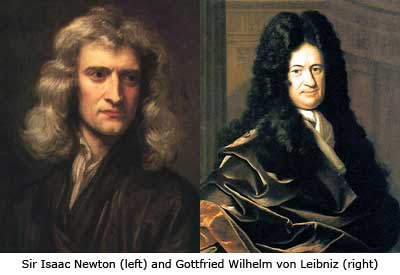
\includegraphics[width=4cm]{./myndir/kafli01/01_NewtonLeibniz.jpg}
 % NewtonLeibniz.jpg: 450x300 pixel, 72dpi, 15.88x10.58 cm, filebb=0 0 450 300
\end{figure}
%}<2>}






\subsubsection*{Ítarefni}
 Fyrir nánari útlistun á hugtökunum sem við fjöllum um þá er hægt að skoða
\begin{itemize}
 \item \href{http://stae.is}{http://stæ.is} (hugtakasafn og orðaskrá)
  \item \href{http://planetmath.org}{http://planetmath.org}
  \item \href{http://mathworld.wolfram.com}{http://mathworld.wolfram.com}
  \item \href{http://en.wikipedia.org}{http://en.wikipedia.org} (ath.~enska útgáfan)
\end{itemize}

\pause
\subsubsection*{Forrit}
 \begin{itemize}
  \item GeoGebra \href{http://www.geogebra.org}{http://www.geogebra.org}
  \item WolframAlpha \href{http://www.wolframalpha.com}{http://www.wolframalpha.com}
 \end{itemize}
\subsection*{Föll}	

\subsubsection*{Tölur}
\begin{enumerate}[(i)]
\item  \emph{Náttúrlegu tölurnar} eru tölurnar
$1, 2, 3, 4, \ldots$ og mengi þeirra er táknað með $\N$.   \pause
\item Mengi \emph{heiltalna} er táknað með $\Z$. $\Z = \ldots,-2,-1,0,1,2,3,\ldots$\pause
\item Mengi \emph{ræðra talna} er táknað með $\Q$. $\Q = \{ \frac pq ; p,q \in \Z \}$.\pause
\item Mengi \emph{rauntalna} er táknað með $\R$.\pause
\item Mengi \emph{tvinntalna} er táknað með $\C$.
\end{enumerate}


\pause

\paragraph{Athugasemd}  
Margir vilja telja $0$ með sem náttúrlega tölu.  Það er eðlilegt ef 
maður lítur á náttúrlegu tölurnar þannig að þær tákni fjölda.  Ef maður lítur hins vegar þannig
á að þær séu notaðar til að númera hluti
þá er 0 ekki með.





\paragraph{Smíði rauntalna}  Rauntölur eru smíðaðar úr ræðu tölunum
með því að fylla upp í götin. 

\pause

T.d.~eru 
\begin{eqnarray*}
\pi &=& 3,1415926\ldots, \qquad \text{og}\\
\sqrt 2 -4  &=& -2,58578\ldots
\end{eqnarray*}
ekki ræðar tölur (það er ekki hægt að skrifa þær sem brot $\frac ab$, 
þar sem $a$ og $b$ eru heilar tölur), en þær eru rauntölur.


\pause


\subsubsection*{Frumsendan um efra mark}  
Látum $A$ vera mengi af  rauntölum
sem er þannig að til er tala $x$, þannig að 
fyrir allar tölur $a \in A$ þá er 
$$a\leq x.$$ 
Þá er til rauntala $x_0$ sem kallast {\em minnsta efra mark} fyrir
$A$, sem er þannig að  $a\leq x_0$ fyrir allar tölur $a\in
A$ og ef $x<x_0$ þá er til tala $a\in A$ þannig að $a>x$.  




\subsubsection*{Bil}
Látum $a$ og $b$ vera rauntölur þannig að $a<b$.  
Skilgreinum 

(i) {\em opið bil}\ \ $(a,b)=\{x\in \R ; a<x<b\}$

(ii) {\em lokað bil}\ \ $[a,b]=\{x\in \R ; a\leq x\leq b\}$

(iii) {\em hálf opið bil}\ \ $[a,b)=\{x\in \R ; a\leq x<b\}$

(iv) {\em hálf opið bil}\ \ $(a,b]=\{x\in \R ; a< x\leq b\}$

\medskip

Þessi bil sem er skilgreind hér fyrir ofan eru kölluð endanleg.  Til
eru fleiri gerðir af bilum:


(v)  {\em opið óendanlegt bil}\ \    $(a,\infty)=\{x\in \R ; a<x\}$

(vi)  {\em opið óendanlegt bil}\ \    $(-\infty, a)=\{x\in \R ; x<a\}$

(vii)  {\em lokað óendanlegt bil} \ \ $[a,\infty)=\{x\in \R ; a\leq x\}$

(viii)  {\em lokað óendanlegt bil}\ \  $(-\infty, a]=\{x\in \R ; x\leq a\}$

(ix)  {\em allur rauntalnaásinn}\ \  $(-\infty, \infty)$.




\paragraph{Skilgreining} Mengi $A$ af rauntölum kallast bil ef um
allar tölur $a<b$ sem eru í menginu $A$ gildir að ef $a<x<b$ þá er $x$
líka í menginu $A$. \pause Þ.e.~\emph{engin göt}.


\pause

\paragraph{Athugasemd}  

(i) Sérhvert bil á rauntalnaásnum er af
einni þeirra gerða sem talin er upp í Skilgreiningu 1.5.   (Þessi
staðhæfing er jafngild frumsendunni um efra mark.)

\pause

(ii) Það er jafngilt að segja 
$$x \in (a-\eta,a+\eta)$$ 
og 
$$|x-a| < \eta.$$



\subsubsection*{Vörpun}
\paragraph{Skilgreining}
\emph{Vörpun} frá mengi $X$ yfir í mengi $Y$ er regla sem úthlutar sérhverju
staki $x$ í $X$ nákvæmlega einu staki $f(x)$ í $Y$. Táknum þetta með
$f:X \to Y$. 

Stakið $f(x)$ kallast \emph{gildi} vörpunarinnar (í punktinum $x$).


\pause

\paragraph{Skilgreining}
Mengið $X$ kallast \emph{skilgreiningarmengi} $f$, 
mengið $Y$ kallast \emph{bakmengi} $f$ og 
mengið $f(X) = \{ f(x); x \in X \}$ kallast \emph{myndmengi} $f$.


\begin{center}
 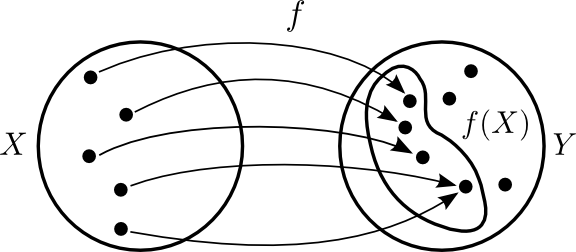
\includegraphics[width=7cm,keepaspectratio=true]{./myndir/kafli01/02_Mynd_vorpunar.png}
 % Mynd_vorpunar.eps: 277x122 pixel, 300dpi, 2.35x1.03 cm, bb=0 0 277 122
\end{center}


\subsubsection*{Samskeyting}
%\paragraph{1.10 Skilgreining}
Látum $f:X \to Y$ og $g:Y \to Z$ vera varpanir. Vörpunin 
$g\circ f:X \to Z$ sem skilgreind er með 
$(g\circ f)(x)=g(f(x))$ kallast \emph{samskeyting} $f$ og 
$g$. 
Stakið 
$g(f(x)) \in Z$ fæst með því að beita fyrst vörpuninni $f$ á stakið 
$x$ og síðan vörpuninni $g$ á stakið $f(x)$.

% {\only{
% \begin{center}
%  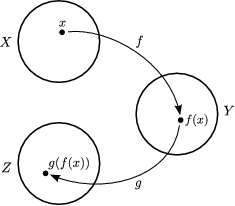
\includegraphics[width=4cm,keepaspectratio=true]{./myndir/kafli01/02_Samskeyting0.png}
%  % Mynd_vorpunar.eps: 277x122 pixel, 300dpi, 2.35x1.03 cm, bb=0 0 277 122
% \end{center}}<1>}
% \pause
% 
% {\only{
\begin{center}
 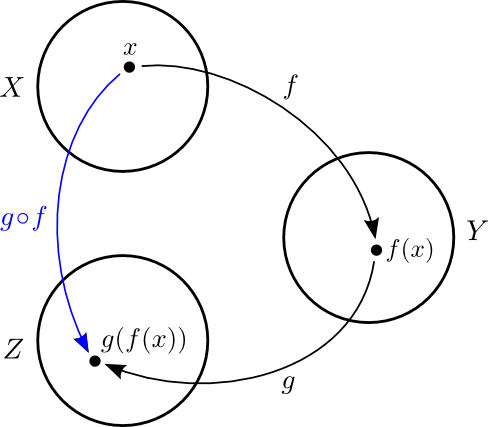
\includegraphics[width=4cm,keepaspectratio=true]{./myndir/kafli01/02_Samskeyting.png}
 % Mynd_vorpunar.eps: 277x122 pixel, 300dpi, 2.35x1.03 cm, bb=0 0 277 122
\end{center}
% }<2>}



\subsubsection*{Eintækni/átækni}
%\paragraph{1.11 Athugasemd}
Það er ekki víst að öll gildin í $Y$ séu tekin (þ.e.~$f(X)$
getur verið minna en $Y$). Eins þá er mögulegt að $f$
taki sama gildið oftar en einu sinni.


\pause

\paragraph{Skilgreining}
Við segjum að vörpunin $f$ sé \emph{átæk} ef $f(X)=Y$, það þýðir að 
fyrir sérhvert stak $y$ í $Y$ þá er til (amk.~eitt) stak
$x$ í $X$ þannig að $f(x)=y$.

\pause

Segjum að vörpunin $f$ sé \emph{eintæk} ef $f(x_1) = f(x_2)$ 
hefur í för með sér að $x_1=x_2$, þ.e.~sérhvert gildi sem
vörpunin tekur er bara tekið einu sinni.


\begin{center}
 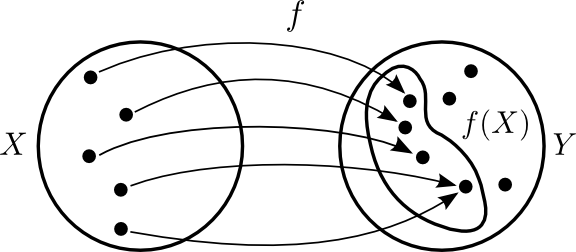
\includegraphics[width=6cm,keepaspectratio=true]{./myndir/kafli01/02_Mynd_vorpunar.png}
 % Mynd_vorpunar.eps: 277x122 pixel, 300dpi, 2.35x1.03 cm, bb=0 0 277 122
\end{center}



\subsubsection*{Andhverfa}
 \paragraph{Skilgreining}
  Vörpun sem er bæði eintæk og átæk kallast \emph{gagntæk}.
 

 \pause
 
\paragraph{Setning}
 Látum $f:X \to Y$ vera vörpun. Sagt er að 
$f$ sé andhverfanleg ef til er vörpun 
$f^{-1}:Y \to X$
þannig að samskeyting varpananna $f$ og 
$f^{-1}$ annars vegar og 
$f^{-1}$ og 
$f$ hins vegar sé viðeigandi 
samsemdarvörpun, þ.e.~$f^{-1}\circ f=id_X$ og
$f\circ f^{-1} = id_Y$.


% {\only{
% \begin{center}
%  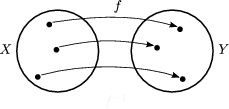
\includegraphics[width=7cm,keepaspectratio=true]{./myndir/kafli01/02_Andhverfa0.png}
%  % Mynd_vorpunar.eps: 277x122 pixel, 300dpi, 2.35x1.03 cm, bb=0 0 277 122
% \end{center}}<1>}
% 
% \pause
% 
% {\only{
\begin{center}
 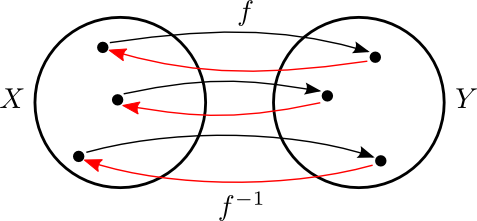
\includegraphics[width=7cm,keepaspectratio=true]{./myndir/kafli01/02_Andhverfa.png}
 % Mynd_vorpunar.eps: 277x122 pixel, 300dpi, 2.35x1.03 cm, bb=0 0 277 122
\end{center}
% }<2>}



\subsubsection*{Graf}
\paragraph{Athugasemd}
 Venjulega hjá okkur þá eru mengin $X$ og $Y$ mengi af rauntölum. Þegar $Y$ er
mengi af tölum þá er notast við orðið \emph{fall} í stað orðsins 
\emph{vörpun}.


\pause

\paragraph{Skilgreining}
Látum $f:X \to Y$ vera fall þannig að $X$ og $Y$ eru mengi 
af rauntölum. \emph{Graf} fallsins $f$ er þá mengi allra punkta í planinu
$\R^2$ af gerðinni $(x,f(x))$ þar sem $x\in X$. 
Notum oft $y$ í stað $f(x)$.


\begin{center}
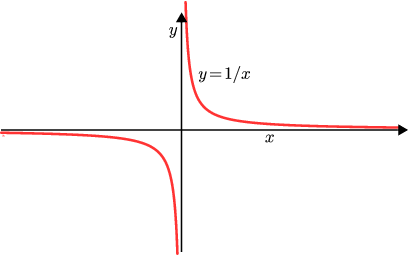
\includegraphics[width=7cm,keepaspectratio=true]{./myndir/kafli01/02_Graf.png}
 % Mynd_vorpunar.eps: 277x122 pixel, 300dpi, 2.35x1.03 cm, bb=0 0 277 122
\end{center}



\subsection*{Markgildi}

\subsubsection*{Óformleg skilgreining}  
%Gerum ráð fyrir að fall $f$ sé
%skilgreint á opnu bili umhverfis punktinn $a$, nema hvað hugsanlega er
%$f(a)$ ekki skilgreint.  
Segjum að  $f(x)$
{\it stefni á tölu $L$ þegar $x$ stefnir á $a$}, og ritum
$\lim_{x\rightarrow a} f(x)=L$, ef við getum tryggt að  $f(x)$ sé {\em
  eins nálægt}
$L$ og við viljum bara með því að velja $x$ {\em nógu nálægt} $a$.  


\pause

\subsubsection*{Skilgreining} Gerum ráð fyrir að fall $f$ sé
skilgreint á opnu bili umhverfis punktinn $a$, nema hvað hugsanlega er
$f(a)$ ekki skilgreint. \pause 
Við segjum að $f(x)$
\emph{stefni á tölu $L$ þegar $x$ stefnir á $a$}, og ritum
$\lim_{x\rightarrow a} f(x)=L$, ef eftirfarandi skilyrði er uppfyllt:

\emph{Fyrir sérhverja tölu $\epsilon>0$ er til tala $\delta>0$ 
þannig að um öll $x$ þannig að}
$$
0<|x-a|<\delta,\quad \text{ þá er } \quad |f(x)-L|<\epsilon.
$$


\pause

\subsubsection*{Athugasemd}  Þegar athugað er hvort markgildið
$\lim_{x\rightarrow a} f(x)$ er til og hvert gildi þess er þá skiptir
ekki máli hvort $f(a)$ er skilgreint eða ekki.



\subsubsection*{Markgildi frá hægri}
%\paragraph{Óformleg skilgreining}   
Gerum ráð fyrir að fall $f$ sé
skilgreint á opnu bili $(a,b)$.  Segjum að  $f(x)$
{\it stefni á tölu $L$ þegar $x$ stefnir á $a$ frá hægri}, og ritum
$\lim_{x\rightarrow a^+} f(x)=L$, ef við getum tryggt að  $f(x)$ sé 
{\em eins nálægt}
$L$ og við viljum bara með því að velja $x>a$ {\em nógu nálægt} $a$. 


\pause

\paragraph{Skilgreining} Gerum ráð fyrir að fall $f$ sé
skilgreint á opnu bili $(a,b)$.  Við segjum að $f(x)$
{\it stefni á tölu $L$ þegar $x$ stefnir á $a$ frá hægri}, og ritum
$\lim_{x\rightarrow a^+} f(x)=L$, ef eftirfarandi skilyrði er uppfyllt.

{\it Fyrir sérhverja tölu $\epsilon>0$ er til tala $\delta>0$ þannig
  að um öll $x$ þannig að} 
$$
a<x<a+\delta,\quad \text{ þá er } \quad |f(x)-L|<\epsilon.
$$



\subsubsection*{Markgildi frá vinstri}
%\paragraph{Óformleg skilgreining}   
Gerum ráð fyrir að fall $f$ sé
skilgreint á opnu bili $(b,a)$.  Segjum að  $f(x)$
{\it stefni á tölu $L$ þegar $x$ stefnir á $a$ frá vinstri}, og ritum
$\lim_{x\rightarrow a^-} f(x)=L$, ef við getum tryggt að  $f(x)$ sé 
{\em eins nálægt}
$L$ og við viljum bara með því að velja $x<a$ {\em nógu nálægt} $a$. 


\pause

\paragraph{Skilgreining} Gerum ráð fyrir að fall $f$ sé
skilgreint á opnu bili $(b,a)$.  Við segjum að $f(x)$
{\it stefni á tölu $L$ þegar $x$ stefnir á $a$ frá vinstri}, og ritum
$\lim_{x\rightarrow a^-} f(x)=L$, ef eftirfarandi skilyrði er uppfyllt.

{\it Fyrir sérhverja tölu $\epsilon>0$ er til tala $\delta>0$ þannig
  að um öll $x$ þannig að} 
$$
a-\delta<x<a,\quad \text{ þá er } \quad |f(x)-L|<\epsilon.
$$



\subsubsection*{Setning} Gerum ráð fyrir að fall $f$ sé
skilgreint á opnu bili umhverfis punktinn $a$, nema hvað hugsanlega er
$f(a)$ ekki skilgreint.  Þá er 
$$\lim_{x\rightarrow a} f(x)=L$$
ef og aðeins ef 
$$\lim_{x\rightarrow a^-} f(x)=L=\lim_{x\rightarrow a^+} f(x).$$




% \subsubsection*{Reiknireglur fyrir markgildi}
% \paragraph{1.12 Setning.}   Gerum ráð fyrir að
% $\lim_{x\rightarrow a}f(x)=L$ og að   $\lim_{x\rightarrow a}g(x)=M$.
% Þá gildir
% 
% (i)\ \ $\lim_{x\rightarrow a}\Big(f(x)+g(x)\Big)=L+M$;
% 
% (ii)\  \ $\lim_{x\rightarrow a}\Big(f(x)-g(x)\Big)=L-M$;
% 
% (iii)\ \  $\lim_{x\rightarrow a}f(x)g(x)=LM$;
% 
% (iv)\ \  $\lim_{x\rightarrow a}kf(x)=kL$, þar sem $k$ fasti;
% 
% (v)\ \  $\lim_{x\rightarrow a}f(x)/g(x)=L/M$, að því gefnu að $M\neq 0$;
% 
% (vi)\ \ Gerum ráð fyrir að $m$ og $n$ séu 
% heiltölur þannig að $f(x)^{m/n}$ sé
%   skilgreint fyrir öll $x$ á bili $(b,c)$ umhverfis $a$ (en ekki
%   endilega fyrir $x=a$) og að $L^{m/n}$ sé skilgreint.
% Þá er $\lim_{x\rightarrow a}f(x)^{m/n}=L^{m/n}$.
% 
% (vii)\ \   Ef til er bil $(b,c)$ sem inniheldur $a$ þannig að 
% $f(x)\leq g(x)$ fyrir öll $x\in (b,c)$, nema kannski $x=a$, þá er
%  $\lim_{x\rightarrow a}f(x)=L\leq M=\lim_{x\rightarrow a}g(x)$.
% 
% 

% \subsubsection*{Klemmureglan}
% \paragraph{1.13 Setning.}Gerum ráð fyrir að $f(x)\leq
% g(x)\leq h(x)$ fyrir öll $x$ á bili $(b, c)$ sem
% inniheldur $a$, nema kannski $x=a$.  Gerum enn fremur ráð fyrir að 
% $$\lim_{x\rightarrow a}f(x)=\lim_{x\rightarrow a}h(x)=L.$$
% Þá er $\lim_{x\rightarrow a}g(x)=L$.
% 
% 



\subsubsection*{Önnur efnisatriði sem þið þurfið að skoða}

\begin{itemize}
\item Jafna línu, P.2
\item Jafna hrings, P.3
 \item Hliðrun og skölun grafs, P.3
 \item (Stranglega) minnkandi og (stranglega) vaxandi föll, 2.8
 \item Jafnstæð og oddstæð föll, P.4
\end{itemize}

 


\lecture[2]{2. Markgildi og samfelldni }{lecture-text}
\date{3.~september 2012}

\maketitle

%\subsection*{Markgildi}

\subsubsection*{Algeng markgildi}
\paragraph{Dæmi}
	\begin{itemize}
	\item $\lim_{x \to a} c = c$, $c$ fasti
	\pause
	\item $\lim_{x \to a} x = a$
	\item $\lim_{x \to a} |x| = |a|$
	\pause
	\item $\lim_{x \to 0} \frac{|x|}{x}$ er ekki til
	\pause
	\item $\lim_{x \to 0^-} \frac{|x|}{x} = -1$
	\item $\lim_{x \to 0^+} \frac{|x|}{x} = 1$
	\end{itemize}



\subsubsection*{Reiknireglur fyrir markgildi}
\pause
 \paragraph{Setning}
   Gerum ráð fyrir að
$\lim_{x\rightarrow a}f(x)=L$ og að   $\lim_{x\rightarrow a}g(x)=M$.
Þá gildir

\pause

(i)\ \ $\lim_{x\rightarrow a}\Big(f(x)+g(x)\Big)=L+M$;

(ii)\  \ $\lim_{x\rightarrow a}\Big(f(x)-g(x)\Big)=L-M$;

\pause

(iii)\ \  $\lim_{x\rightarrow a}f(x)g(x)=LM$;

(iv)\ \  $\lim_{x\rightarrow a}kf(x)=kL$, þar sem $k$ fasti;

(v)\ \  $\lim_{x\rightarrow a}f(x)/g(x)=L/M$, að því gefnu að $M\neq 0$;

\pause

(vi)\ \ Gerum ráð fyrir að $m$ og $n$ séu 
heiltölur þannig að $f(x)^{m/n}$ sé
  skilgreint fyrir öll $x$ á bili $(b,c)$ umhverfis $a$ (en ekki
  endilega fyrir $x=a$) og að $L^{m/n}$ sé skilgreint.
Þá er $\lim_{x\rightarrow a}f(x)^{m/n}=L^{m/n}$.

\pause

(vii)\ \   Ef til er bil $(b,c)$ sem inniheldur $a$ þannig 
að $f(x)\leq g(x)$ fyrir öll $x\in (b,c)$, nema kannski $x=a$, þá 
er $\lim_{x\rightarrow a}f(x)=L\leq M=\lim_{x\rightarrow a}g(x)$.

 


\subsubsection*{VARÚÐ}
%\paragraph{Athugasemd}
	Liður (i) í setningunni á undan segir að ef markgildin
	$\lim_{x\to a} f(x)$ og $\lim_{x\to a} g(x)$ eru til þá
	sé markgildið
	$\lim_{x\to a} (f(x)+g(x))$ einnig til.

\bigskip\pause

	En hún segir {\bf ekki} að ef 
	$f$ og $g$ eru föll þannig að markgildið
	$\lim_{x\to a} (f(x)+g(x))$ er til, að þá séu markgildin
	$\lim_{x\to a} f(x)$ og $\lim_{x\to a} g(x)$ einnig til.





\subsubsection*{Klemmureglan}

\pause

\paragraph{(iv)-liður í setningu 2.2 að ofan}
Ef til er bil $(b,c)$ sem inniheldur $a$ þannig að 
$f(x)\leq g(x)$ fyrir öll $x\in (b,c)$, nema kannski $x=a$, þá er
 $\lim_{x\rightarrow a}f(x)=L\leq M=\lim_{x\rightarrow a}g(x)$.


\pause

\paragraph{Setning.}  Gerum ráð fyrir að $f(x)\leq
h(x)\leq g(x)$ fyrir öll $x$ á bili $(b, c)$ sem
inniheldur $a$, nema kannski $x=a$.  Gerum enn fremur ráð fyrir að 
$$\lim_{x\rightarrow a}f(x)=\lim_{x\rightarrow a}g(x)=L.$$

\pause

Þá er $\lim_{x\rightarrow a}h(x)=L$.
 



%\subsubsection*{Skiladæmi}
% \paragraph{Frágangur skiladæma}
% \begin{itemize}
% \item Skrifið upp {\bf dæmið} og lausnina snyrtilega
% \pause
% \item Vísið í setningar sem þið notið
% \pause
% \item Notið ekki rökfræðitákn eins og $\Leftarrow$, 
% $\Rightarrow$, $\Leftrightarrow$, $\wedge$, $\vee$
% \pause
% \item Textinn á að vera samfelldur og læsilegur (lesið hann 
% sjálf yfir)
% \pause
% \item Skýrt svar/niðurstaða
% \end{itemize}
 
 
% \pause
% \emph{"Forty-two!" yelled Loonquawl. "Is that all you've got to show 
% for seven and a half million years' work?"}
% 
% \emph{"I checked it very thoroughly," said the computer, "and that 
% quite definitely is the answer. I think the problem, to be quite 
% honest with you, is that you've never actually known what the 
% question is."} \hfill -Douglas Adams
 


\subsubsection*{Önnur efnisatriði sem þið þurfið að skoða}

\begin{itemize}
\item Margliður; deiling, þáttun og rætur, P.6
\item Tölugildisfallið, P.1
\item Þríhyrningsójafnan, P.1
 \item Formerkjafallið, $sgn(x)$, P.5
\end{itemize}

 

\lecture[3]{3. Markgildi og samfelldni}{lecture-text}
\date{5.~september 2012}


	\maketitle


\subsection*{Mikilvæg markgildi}



%\subsection*{Markgildi í $-\infty$ og $\infty$}
\subsubsection*{Markgildi þegar $x$ stefnir á $\infty$}
%  {\only{
\begin{center}
 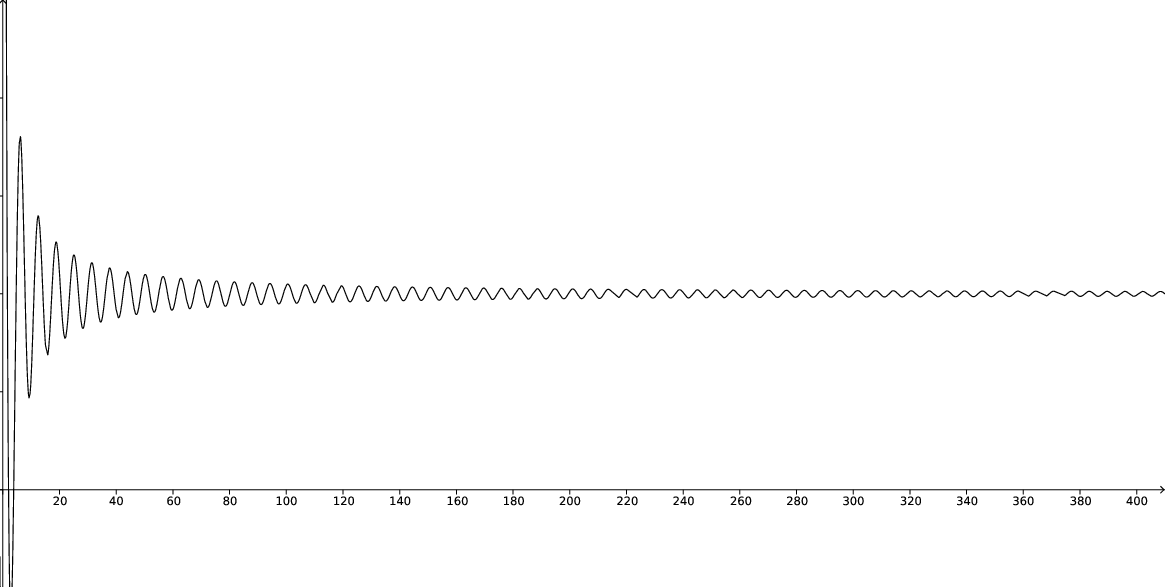
\includegraphics[width=8cm,keepaspectratio=true]{./myndir/kafli01/03_liminf.png}
 % Mynd_vorpunar.eps: 277x122 pixel, 300dpi, 2.35x1.03 cm, bb=0 0 277 122
\end{center}
%}<1,2>}
\pause
 %\paragraph{3.1 Óformleg skilgreining}
 Gerum ráð fyrir að fall $f$ sé
skilgreint á bili $(a, \infty)$.  Segjum að  $f(x)$
{\it stefni á tölu $L$ þegar $x$ stefnir á $\infty$}, og ritum
$\lim_{x\rightarrow \infty} f(x)=L$, ef við getum tryggt að  $f(x)$ sé eins
{\em nálægt}
$L$ og við viljum bara með því að velja $x$ {\em nógu stórt}.
 


%\subsubsection*{Markgildi þegar $x$ stefnir á $\infty$ (framh)}
\paragraph{Skilgreining}
 Gerum ráð fyrir að fall $f$ sé
skilgreint á bili $(a,\infty)$.  Við segjum að $f(x)$
{\it stefni á tölu $L$ þegar $x$ stefnir á $\infty$}, og ritum
$\lim_{x\rightarrow \infty} f(x)=L$, ef eftirfarandi skilyrði er uppfyllt

{\it fyrir sérhverja tölu $\epsilon>0$ er til tala $R$ þannig
  að um öll $R<x$ } 

{\em gildir að  $|f(x)-L|<\epsilon$.}




\subsubsection*{Markgildi þegar $x$ stefnir á $-\infty$}
Fyrir $-\infty$ er þetta gert með sama sniði.

%  \paragraph{3.3 Óformlega skilgreining}
 Gerum ráð fyrir að fall $f$ sé
skilgreint á bili $(-\infty, a)$.  Segjum að  $f(x)$
{\it stefni á tölu $L$ þegar $x$ stefnir á $-\infty$}, og ritum
$\lim_{x\rightarrow -\infty} f(x)=L$, ef við getum tryggt að  $f(x)$ sé eins
{\em nálægt}
$L$ og við viljum bara með því að velja $x$ sem {\em nógu stóra} 
mínus tölu.
 

 \pause
 
\paragraph{Skilgreining}
Gerum ráð fyrir að fall $f$ sé
skilgreint á bili $(-\infty,a)$.  Við segjum að $f(x)$
{\it stefni á tölu $L$ þegar $x$ stefnir á $-\infty$}, og ritum
$\lim_{x\rightarrow -\infty} f(x)=L$, ef eftirfarandi skilyrði er uppfyllt

{\it fyrir sérhverja tölu $\epsilon>0$ er til tala $R$ þannig
  að um öll $x<R$ } 

{\em gildir að  $|f(x)-L|<\epsilon$.} 




\subsubsection*{$\infty$ sem markgildi}
 %\paragraph{3.5 Óformleg skilgreining.} 
 Gerum ráð fyrir að fall $f$ sé
skilgreint á opnu bili umhverfis punktinn $a$, nema hvað hugsanlega er
$f(a)$ ekki skilgreint.  Segjum að  $f(x)$
{\it stefni á $\infty$ þegar $x$ stefnir á $a$}, og ritum
$\lim_{x\rightarrow a} f(x)=\infty$, ef við getum tryggt að  $f(x)$ sé {\em
  hversu stórt sem við viljum}
 bara með því að velja $x$ {\em nógu nálægt} $a$.  

 
\pause
\paragraph{Skilgreining}
 Gerum ráð fyrir að fall $f$ sé
skilgreint á opnu bili umhverfis punktinn $a$, nema hvað hugsanlega er
$f(a)$ ekki skilgreint.  Við segjum að $f(x)$
{\it stefni á $\infty$ þegar $x$ stefnir á $a$}, og ritum
$\lim_{x\rightarrow a} f(x)=\infty$, ef eftirfarandi skilyrði er uppfyllt

{\it fyrir sérhverja tölu $B$ er til tala $\delta>0$ þannig
  að um öll $x$ þannig að} 

{\em $0<|x-a|<\delta$ 
gildir að  $f(x)>B$.}




\subsubsection*{Málvenja}
 %\paragraph{3.7 Athugasemd.} 
 Athugið að $\infty$ er {\bf ekki} tala.  Þó 
að  $\lim_{x\rightarrow a} f(x)=\infty$ þá er samt sagt að
markgildið $\lim_{x\rightarrow a} f(x)$ sé ekki til.
 


\subsubsection*{$-\infty$ sem markgildi}
% \paragraph{3.8 Óformleg skilgreining.} 
 Gerum ráð fyrir að fall $f$ sé
skilgreint á opnu bili umhverfis punktinn $a$, nema hvað hugsanlega er
$f(a)$ ekki skilgreint.  Segjum að  $f(x)$
{\it stefni á $-\infty$ þegar $x$ stefnir á $a$}, og ritum
$\lim_{x\rightarrow a} f(x)=-\infty$, ef við getum tryggt að  $f(x)$ sé {\em
  hversu lítið sem við viljum}
 bara með því að velja $x$ {\em nógu nálægt} $a$.  

 
\pause
\paragraph{Skilgreining}
 Gerum ráð fyrir að fall $f$ sé
skilgreint á opnu bili umhverfis punktinn $a$, nema hvað hugsanlega er
$f(a)$ ekki skilgreint.  Við segjum að $f(x)$
{\it stefni á $-\infty$ þegar $x$ stefnir á $a$}, og ritum
$\lim_{x\rightarrow a} f(x)=-\infty$, ef eftirfarandi skilyrði er uppfyllt

{\it fyrir sérhverja tölu $B$ er til tala $\delta>0$ þannig
  að um öll $x$ þannig að} 

{\em $0<|x-a|<\delta$ 
gildir að  $f(x)<B$.}




\subsubsection*{Málvenja}
% \paragraph{3.10 Athugasemd.}  
Athugið að $-\infty$ er {\bf ekki} tala.  Þó 
að  $\lim_{x\rightarrow a} f(x)=-\infty$ þá er samt sagt að
markgildið $\lim_{x\rightarrow a} f(x)$ sé ekki til.
 


\subsubsection*{Markgildi með $\sin$}
\paragraph{Sýnidæmi}
\begin{itemize}
  \item $$\lim_{x\to 0} \sin\left(\frac 1x\right) \quad \text{er ekki til}$$
  \pause
  \item $$\lim_{x\to 0} x\sin\left(\frac 1x\right) = 0$$
  \pause
  \item $$\lim_{x \to 0} \frac{\sin(x)}{x} = 1$$
\end{itemize}




\subsection*{Samfelldni}

\subsubsection*{Skilgreining}
Látum $A\subseteq \R$ og $x\in A$.  Við segjum að $x$ sé {\em innri
  punktur} $A$ ef $A$ inniheldur opið bil umhverfis $x$, það er að
segja til er tala $\delta>0$ þannig að $(x-\delta, x+\delta)\subseteq
A$. 

\pause

Ef $x$ er ekki innri punktur $A$ og $x\in A$ þá segjum við að $x$ sé
{\em jaðarpunktur} $A$.

\pause



\subsubsection*{Skilgreining.}
Látum $f$ vera fall og $c$ innri punkt skilgreiningarsvæðis $f$.  Sagt
er að $f$ sé {\em samfellt í punktinum} $c$ ef
$$\lim_{x\rightarrow c}f(x)=f(c).$$



\subsubsection*{Setning}
 Látum $f$ og $g$ vera föll.  Gerum ráð fyrir að $c$ sé innri punktur
skilgreiningarsvæðis beggja fallanna og að bæði föllin séu samfelld í
punktinum $c$.  Þá eru eftirfarandi föll samfelld í $c$:
\begin{itemize}
\pause
\item[(i)] $f+g$ %(Fallið $f+g$ er skilgreint þannig að $(f+g)(x)=f(x)+g(x)$.)
\pause
\item[(ii)] $f-g$
\pause
\item[(iii)] $fg$
\pause
\item[(iv)] $kf$, þar sem $k$ er fasti
\pause
\item[(v)]  $f/g$, ef $g(c)\neq 0$
\pause
\item[(vi)]  $\Big(f(x)\Big)^{1/n}$, að því gefnu að 
$f(c)>0$ ef $n$ er slétt tala og $f(c)\neq 0$ ef $n<0$.
\end{itemize} 



\subsubsection*{Samskeyting samfelldra falla}
 \paragraph{Setning}
 Látum $g$ vera fall sem er skilgreint á opnu bili umhverfis $c$ og
samfellt í $c$ og látum $f$ vera fall sem er skilgreint á opnu bili
umhverfis $g(c)$ og samfellt í $g(c)$.  Þá er fallið $f\circ g$
skilgreint á opnu bili umhverfis $c$ og er samfellt í $c$.  
%[Fallið $f\circ g$ er skilgreint þannig að $(f\circ g)(x)=f(g(x))$ fyrir þau
%gildi á $x$ þar sem bæði $g(x)$ og $f(g(x))$ eru skilgreind.]
% 
% Ef $f$ er samfellt í punkti $L$ og $\lim_{x\rightarrow c}g(x)=L$ þá er
% $$\lim_{x\rightarrow c}f\big(g(x)\big)=f(L)=f\bigg(\lim_{x\rightarrow c}g(x)\bigg).$$
% [Ekki forsenda varðandi þetta síðasta atriði að $g$ sé samfellt í $c$.]
 


\subsubsection*{Hefð}
% \paragraph{Athugasemd}
  Ef fall er skilgreint með formúlu og skilgreingamengið er ekki
tilgreint sérstaklega, þá er venjan að líta alla þá punkta þar
sem formúlan gildir sem skilgreingarmengi fallsins
 


\subsubsection*{Samfelld föll}
% \paragraph{Skilgreining}
 Við segjum að fall $f$ sé \emph{samfellt} ef það er samfellt í sérhverjum
punkti skilgreingarmengisins.


\pause

\paragraph{Dæmi}
Eftirfarandi föll eru samfelld
\begin{itemize}
\pause
  \item[(a)] margliður
\pause
  \item[(b)] ræð föll
\pause
  \item[(c)] ræð veldi
\pause
  \item[(d)] hornaföll; $\sin$, $\cos$, $\tan$
\pause
  \item[(e)] tölugildisfallið $|x|$
\end{itemize}




\subsubsection*{Að búa til samfelld föll}
% \paragraph{3.19 Athugasemd}
 Með því að nota föllin úr Dæmi 3.18 sem efnivið þá getum við búið til 
fjölda samfelldra fall með því að beita aðgerðunum úr Setningu 3.14 og 
Setningu 3.15.
 





\lecture[4]{4. Markgildi og samfelldni II}{lecture-text}
\date{10.~september 2012}

% Samfelldni frá vinstri/hægri
% Samfelldni á lokuðu bili
% Athugasemd

% Há- og lággildislögmálið
% Milligildissetningin
% Fylgisetning: Margliður af oddatölustigi hafa núllstöðvar

% Afleiða falls
% Diffranlegt fall er samfellt
% Samfellt fall er ekki nauðsynlega diffranlegt

% Ítarefni: Samfelldni frá hægri og vinstri
	\maketitle


%\subsection*{Samfelldni}
\subsubsection*{Upprifjun}
	\pause
 \paragraph{Skilgreining}
	Látum $f$ vera fall og $c$ innri punkt skilgreiningarsvæðis $f$.  Sagt
	er að $f$ sé {\em samfellt í punktinum} $c$ ef
	$$\lim_{x\rightarrow c}f(x)=f(c).$$
 
	\pause
 \paragraph{Athugasemd}
	Þessi skilgreining virkað aðeins fyrir innri punkta skilgreiningarsvæðisins.
	Hins vegar getum við útvíkkað skilgreininguna á samfelldni fyrir 
	hægri og vinstri endapunkta bila með því að einskorða okkur
	við markgildi frá vinstri og hægri.
 


\subsubsection*{Hægri/vinstri samfelldni}	
 %\paragraph{4.3 Skilgreining}
		(i)  Fall $f$ er {\em samfellt frá hægri í punkti} $c$ ef
  $\lim_{x\rightarrow c^+}f(x)=f(c)$.
  
Hér er gert ráð fyrir að fallið $f$ sé amk.~skilgreint á bilinu
  $[c, a)$.

\pause
\medskip

\noindent
(ii)  Fall $f$ er {\em samfellt frá vinstri í punkti} $c$ ef
  $\lim_{x\rightarrow c^-}f(x)=f(c)$.
  
  Hér er gert ráð fyrir að fallið $f$ sé amk.~skilgreint á bilinu
  $(a, c]$.

 

\subsubsection*{Samfelld föll}
 \paragraph{Skilgreining (uppfærð)}
 Gerum ráð fyrir að $f$ sé fall sem er skilgreint á
 mengi $A$, þar sem $A$ er sammengi endanlega margra bila.
 Við segjum að fallið $f$ sé \emph{samfellt} ef það er samfellt í 
 öllum innri punktum skilgreingarmengisins, og ef það er samfellt
 frá hægri/vinstri í jaðarpunktum skilgreingarmengisins,
 eftir því sem við á.

\pause
\paragraph{Athugasemd}
	Ef fall er samfellt á opnu bili $(a,b)$, og ef 
	$a<c<d<b$, þá er fallið einnig samfellt á bilinu 
	$[c,d]$.
 


\subsubsection*{Há- og lággildislögmálið}
 \paragraph{Setning}
 Látum $f$ vera samfellt fall skilgreint á lokuðu takmörkuðu bili
  $[a,b]$.  Þá eru til tölur $x_1$ og $x_2$ í $[a,b]$ þannig að 
fyrir allar tölur $x$ í $[a,b]$ er
$$f(x_1)\leq f(x)\leq f(x_2).$$

\pause

Þetta þýðir að samfellt fall $f$ á lokuðu og takmörkuðu
bili $[a,b]$ tekur bæði hæsta og lægsta gildi á bilinu. \pause
Hæsta
gildið er þá $f(x_2)$ og lægsta gildið er $f(x_1)$.


\pause
 
\paragraph{Athugasemd}
 Það er mögulegt að fallið taki há/lággildi
 sitt í fleiri en einum punkti.



\subsubsection*{Milligildissetningin}
 \paragraph{Setning}
 Látum $f$ vera samfellt fall skilgreint á lokuðu takmörkuðu bili
$[a,b]$.  Gerum ráð fyrir að $s$ sé tala sem liggur á milli $f(a)$ og
$f(b)$.  Þá er til tala $c$ sem liggur á milli $a$ og $b$ þannig að
$f(c)=s$. 
 
<iframe scrolling="no" src="https://tube.geogebra.org/material/iframe/id/zEQQcGcQ/width/1075/height/767/border/888888/rc/false/ai/false/sdz/true/smb/false/stb/false/stbh/true/ld/false/sri/true/at/auto" width="1075px" height="767px" style="border:0px;"> </iframe>>
%  {\only{
\begin{center}
 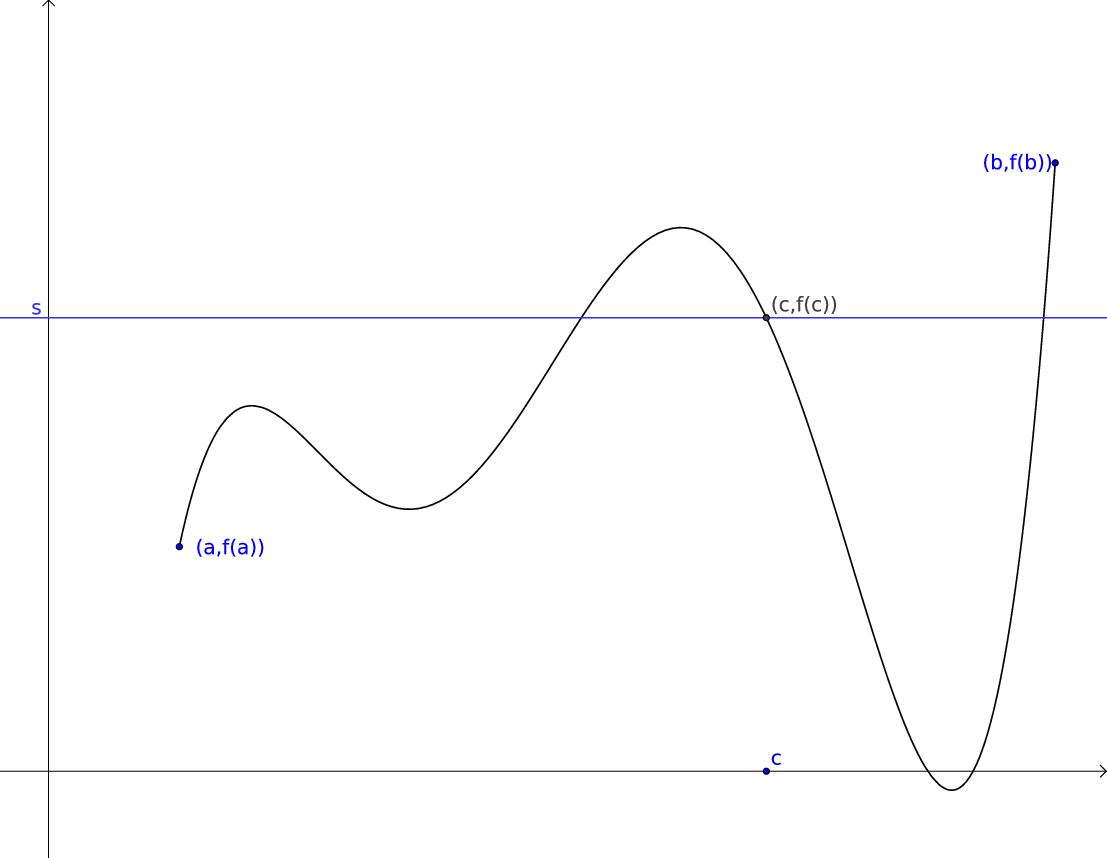
\includegraphics[width=8cm,keepaspectratio=true]{./myndir/kafli01/04_Milligildissetn.png}
 % Mynd_vorpunar-eps-converted-to.pdf: 277x122 pixel, 300dpi, 2.35x1.03 cm, bb=0 0 277 122
\end{center}
%}<1,2>}



 \paragraph{Fylgisetning}
Ef $P(x)=a_nx^n+a_{n-1}x^{n-1}+\cdots+a_1x+a_0$ er margliða af
oddatölu stigi, þá er til rauntala $c$ þannig að $P(c)=0$.
 
 \pause
 \textbf{Sönnun}
	Gerum ráð fyrir að $a_n>0$. \pause
	Þá er $\lim_{x\to -\infty} P(x) = -\infty$ og
	$\lim_{x\to \infty} P(x) = \infty$.\pause
	Það þýður að til eru tölur $a$ og $b$ 
	þannig að $P(a)<0$ og $P(b)>0$. \pause
	Með því að beita Milligildissetningunni á fallið $P$ á 
	bilinu $[a,b]$ og með $s=0$ þá fæst að til er núllstöð 
	á bilinu $[a,b]$.\pause
	
	Ef $a_n < 0$ þá víxlast markgildin að ofan en röksemdafærslan er
	að öðru leyti eins.
	 %þegar $x\to -\infty$ og $x \to \infty$.
 


\end{document}
